\chapter{State of the Art}
\label{state_of_art}
\linenumbers

\lettrine[lines=2]{I}{n traditional IT}, an attacker aims to understand the behavior of a program through various techniques so as to bring attacks aimed at changing its execution flow, functionalities or bypassing limits imposed by the licensing of such software. These attack techniques include a \textbf{preliminary study} of the program: a \textit{static analysis} (i.e., a preliminary analysis of the software without it running) and a \textit{dynamic analysis} (i.e., an analysis performed with the program running).\\
The result of these two preliminary investigation techniques is a \textbf{reverse engineering} of the software, which is useful for identifying any weaknesses or bugs and therefore planning an attack.

\bigskip
In the OT context, however, the concept of \textit{reverse engineering} is also associated with that of \textit{\textbf{process comprehension}}, a term coined by Green et al.'s \cite{green_et_al} to describe the understanding of the characteristics of the system and the physical elements of within it, that are responsible for its proper functioning.

\bigskip
Not much knowledge exists in the literature regarding the collection and analysis of information concerning the understanding and operation of an ICS: in Section \ref{sec:related_work} we will look at a quick overview of some of the existing literature on the subject and in the following sections we will focus in particular on one of the papers exposed.

\vfill

\section{Literature on Process Comprehension}
\label{sec:related_work}
\begin{description}
	\item[Keliris and Maniatikos] The first approach presented in this section is by Keliris and Maniatakos \cite{keliris_maniatakos}: they present a methodology for automating the reverse engineering of ICS binaries based on a \textit{modular framework} (called ICSREF) that can reverse binaries compiled with CODESYS, one of the most popular and widely used PLC compilers, irrespective of the language used.
	
	\item[Yuan et al.] Yuan et al. \cite{yuan_et_al} propose a \textit{data-driven} approach to discovering cyber-physical systems from data directly: to achieve this goal, they have implemented a framework whose purpose is to identify physical systems and transition logic inference, and to seek to understand the mechanisms underlying these cyber-physical systems, making furthermore predictions concerning their state trajectories based on the discovered models.
	
	\item[Feng et al.] Feng et al. \cite{feng_swat} developed a framework that can generate system \textit{invariant rules} based on machine learning and data mining techniques from ICS operational data log. These invariants are then selected by systems engineers to derive IDS systems from them.
	
	The experiment results on two different testbeds, the \textit{Water Distribution system} (WaDi) and the \textit{Secure Water Treatment system} (SWaT), both located at the iTrust - Center for Research in Cyber Security at the University of Singapore \cite{itrust_site}, show that under the same false positive rate invariant-based IDSs have a higher efficiency in detecting anomalies than IDS systems based on a residual error-based model. 
	
	\item[Pal et al.] Pal et al. \cite{pal_et_al} work is somewhat related to Feng et al.'s: this paper describes a data-driven approach to identifying invariants automatically using \textit{association rules mining} \cite{association_rules_mining} with the aim of generate invariants sometimes hidden from the design layout. The study has the same objective of Feng et al.'s and uses too the iTrust SwaT System as testbed.
	
	Currently this technique is limited to only pair wise sensors and actuators: for more accurate invariants generation, the technique adopted must be capable of deriving valid constrains across multiple sensors and actuators.
	
	\item[Winnicki et al.] Winnicki et al. \cite{winnicki_et_al} instead propose a different approach to process comprehension based on the \textbf{attacker's perspective} and not limited to mere \textit{Denial of Service} (DoS): their approach is to discover the dynamic behavior of the system, in a semi-automated and process-aware way, through \textit{probing}, that is, slightly perturbing the cyber physical system and observing how it reacts to changes and how it returns to its original state. The difficulty and challenge for the attacker is to perturb the system in such a way as to achieve an observable change, but at the same time avoid this change being seen as a system anomaly by the IDSs.
	
	\item[Green et al.] Green et al. \cite{green_et_al} also adopt an approach based on the attacker's perspective: this approach consists of two practical examples in a \textit{Man in the Middle} (MitM) scenario to obtain, correlate, and understand all the types of information an attacker might need to plan an attack to alter the process while avoiding detection.
	
	The paper shows \textit{step-by-step} how to perform a ICS \textbf{reconnaissance}, which is fundamental to process comprenension and thus to the execution of MiTM attacks.
	
	\item[Ceccato et al.] Ceccato et al. \cite{ceccato} propose a methodology based on a \textit{black box dynamic analysis} of an ICS using a reverse engineering tool to derive from the scans performed on the memory registers of the exposed PLCs and network scans an approximate model of the physical process. This model is obtained by inferring statistical properties, business process and system invariants from data logs.
	
	The proposed methodology was tested on a non-trivial case study, using a testbed inspired by an industrial water treatment plant.
	
	In the next section I will examine this latest work in more detail, which will be the basis for my work and thus the subsequent chapters of this thesis.

\end{description}

\section{Ceccato et al.’s methodology for analyzing water-tank systems}
\label{sec:ceccato_metodology}
As mentioned earlier, the paper proposes a methodology based on a black box dynamic analysis of an ICS by identifying potential PLCs on the network and scanning the memory registers of the identified controllers to obtain an approximate model of the controlled physical process.

\bigskip
The first objective of this black box analysis is to associate the various memory registers of the target PLCs with a correspondence to the basic concepts of an ICS such as sensors (otherwise known as measurements), actuators, setpoints (range of values of a physical variable), network communications, and so on.\\
This is performed by analyzing the different types of memory registers associated with the Modbus protocol and trying to figure out what type of data they may contain.

The second objective is to put in relation the runtime evolution of these basic concepts.

\bigskip
To achieve this, Ceccato et al. developed a prototype tool \cite{plc_re} that performs reverse engineering of the physical system through four phases:

\begin{enumerate}
	\item \textbf{scanning of the system and data pre-processing}: data gathering is performed to generate the data logs of PLCs registers
	\item \textbf{graphs and statistical analysis}: provides information about the memory registers using graphs and statistical data derived from the gathered data
	\item \textbf{invariant inference and analysis}: generates system invariants and allows user to view invariants related to a given sensor or actuator
	\item \textbf{business process mining}: reconstructs, from event logs, the business process that shows how process is carried out
\end{enumerate}

In Figure \ref{fig:ceccato_overview} we have a schematic representation of the workflow related to this work. We will cover all these phases in detail in the next sections of this chapter. 

\begin{figure}[ht]
	\centering
	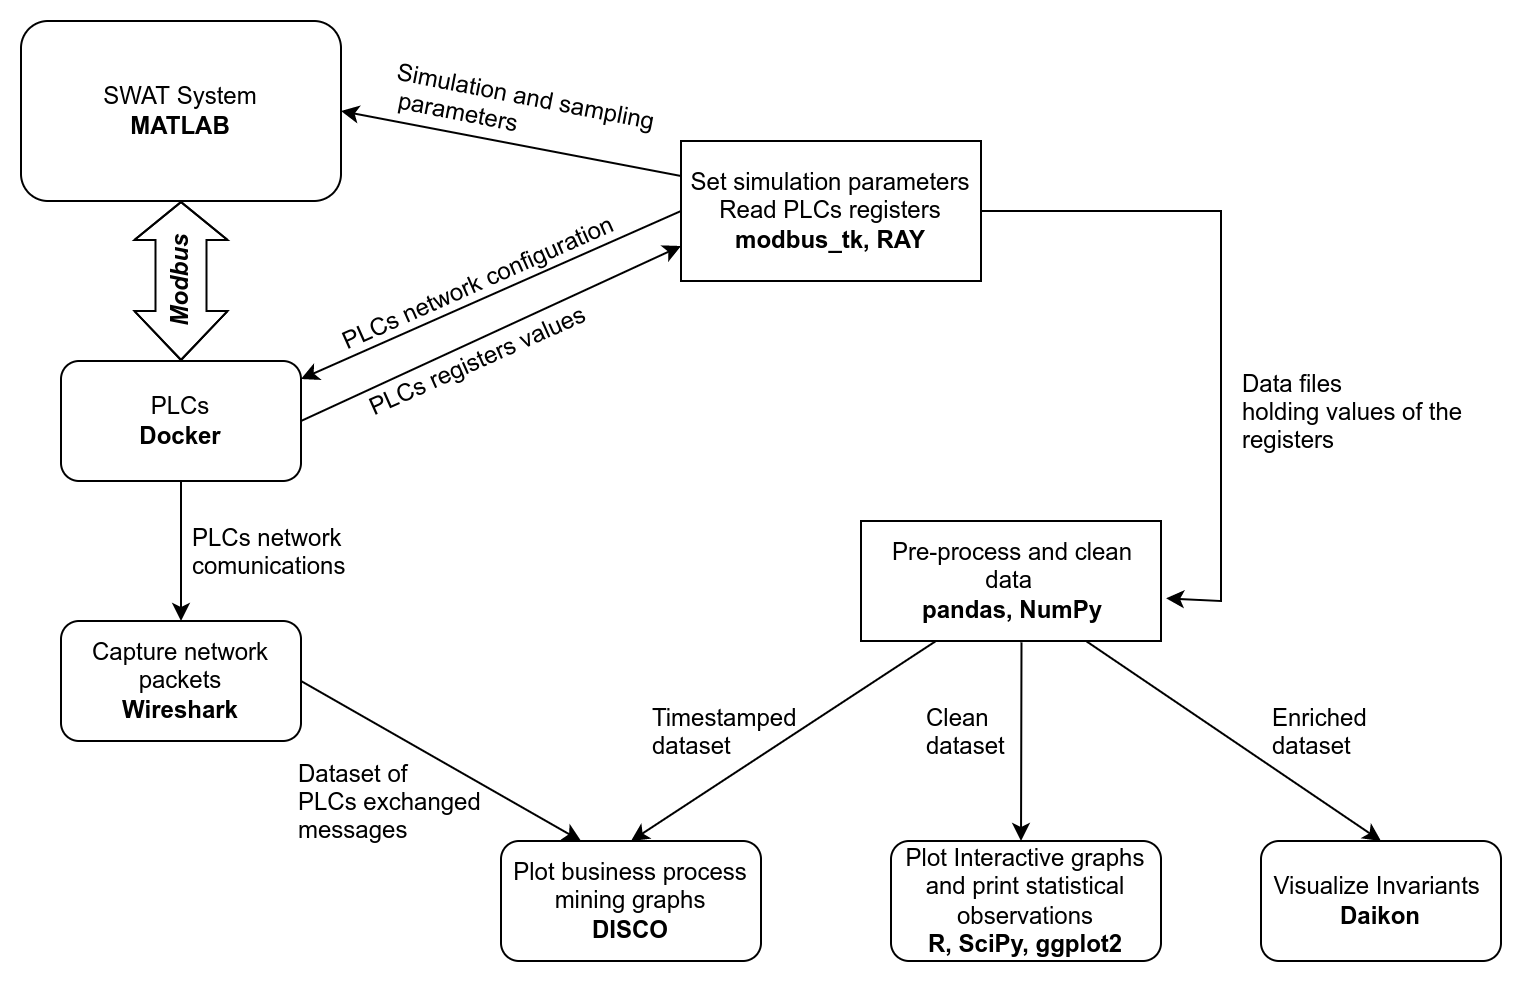
\includegraphics[scale=0.25]{ceccato_flowchart.png}
	\caption{Overview}
	\label{fig:ceccato_overview}
\end{figure}

\subsection{Testbed}
\label{subsec:ceccato_testbed}
Before describing the various phases of the methodology, let's take a look at the testbed on which this methodology will be tested. The testbed used to test this methodology is a (very) simplified version of the iTrust SWaT system \cite{swat_home} implemented by Lanotte et al. \cite{lanotte_et_al}: in Figure 3.2 we can see a graphical representation of the testbed. This simplified version consists of three stages, each controlled by a dedicated PLC: 

\begin{figure}[ht]
	\centering
	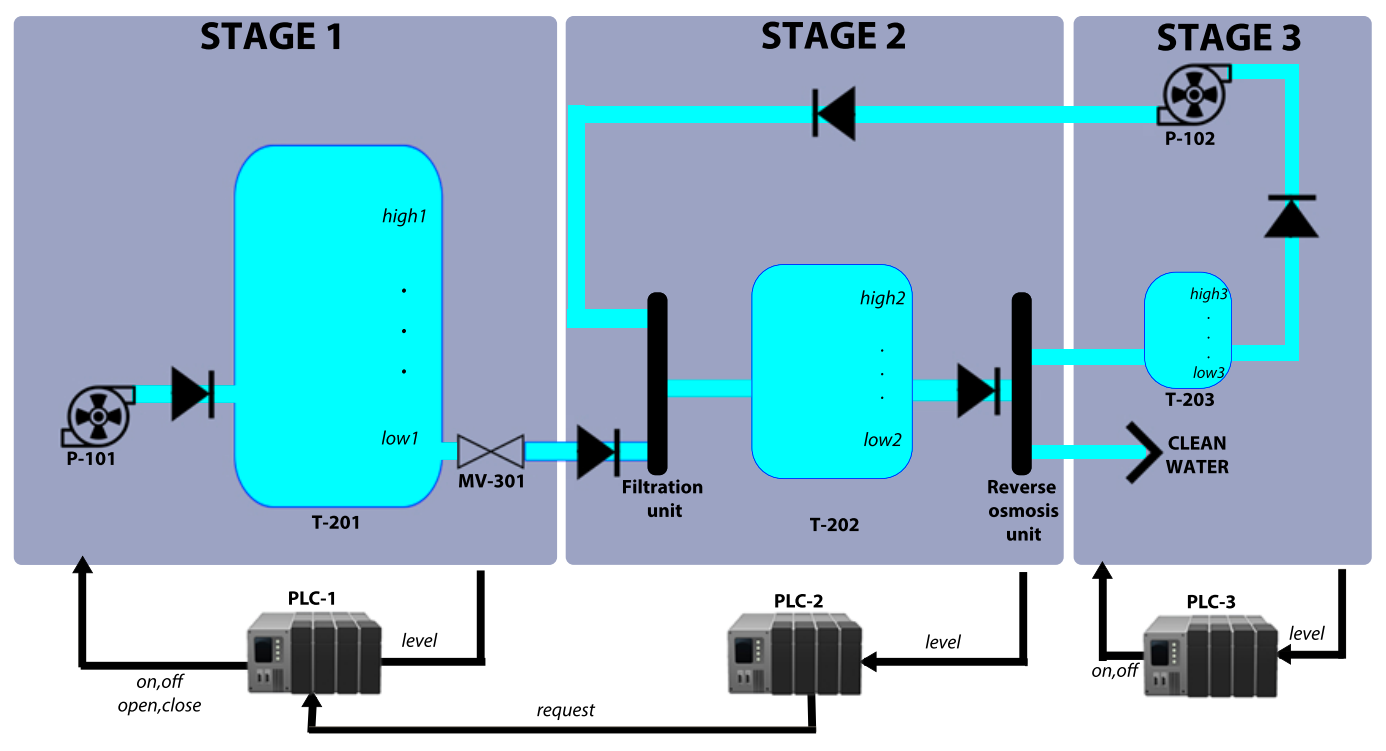
\includegraphics[scale=0.27]{univr_testbed.png}
	\caption{The simplified SWaT system used for running Ceccato et al. methodology}
	\label{fig:univr_testbed}
\end{figure}

\bigskip
\begin{description}
	\item[Stage 1] At the first stage, a \textbf{tank} with a capacity of 80 gallons (identified by the code T-201) is filled with raw water by the P-101 pump: the MV-301 valve (where MV stands for \textit{motorized valve}), also connected to the T-201 tank, flushes out the water collected in the tank to send it to the second stage, first to the \textit{filtration unit} (here not identified by any sensor) and from there to a \textbf{second tank}, identified by the code T-202 and with a capacity of 20 gallons.
	
	\item[Stage 2] At the second stage, water contained in T-202 flows into the \textit{reverse osmosit unit} (RO, which in this case also acts as a valve, extracting water continuously: however, it is not identified as a pump) to reduce organic impurities in the same water. The water then flows from the \textit{RO unit} to the third and last stage.
	
	\item[Stage 3] At the third stage, the water from the \textit{RO unit} is divided according to whether standards are met: if the water is clean it will be fed into the distribution system, otherwise it will go to a \textit{backwash tank}, identified by code T-203 and a capacity of one gallon. The water in this tank will then be pumped back to the stage 2 \textit{filtration unit} through pump P-102.
\end{description}

\bigskip
As mentioned, each stage corresponds to a PLC that controls it, PLC1, PLC2 and PLC3, respectively. Let us briefly see the behavior of each of them:

\begin{description}
	\item[PLC1] PLC1 checks the level of tank T-201 distinguishing three cases:
	
	\begin{itemize}
		\item if T-201 reaches the \textit{low setpoint low1} (hardcoded in memory registers), pump \textbf{P-101 is opened} and valve \textbf{MV-301 is closed}, so that the tank can be filled
		
		\item if T-201 reaches \textit{high setpoint high1} (also hardcoded in the memory registers), pump \textbf{P-101 is closed}
		
		\item in intermediate cases, \textbf{PLC1 waits for request from PLC2} to open/close valve MV-301: if a request to open the valve MV-301 arrives, water will flow from T-201 to T-202, otherwise the valve is closed. In both situations, pump P-101 remains closed 
	\end{itemize}

	\item[PLC2] PLC2 monitors the level of tank T-202, behaving accordingly depending on the level of water in it. Here again there are three cases to consider:
	
	\begin{itemize}
		\item if the water level reaches the \textit{low setpoint low2} (also hardcoded in the memory registers), PLC2 sends a request to PLC1 via a Modbus channel to \textbf{open valve MV-301} in order to flow water from tank T-201 to tank T-202. The transmission channel is implemented by copying a boolean value from a memory register of PLC2 to a corresponding register of PLC1
		
		\item if the water level reaches the \textit{high setpoint high2} instead (hardcoded in the memory registers as the previous setpoints), PLC2 sends PLC1 a \textbf{close request} for valve MV-301
		
		\item In intermediate cases, the valve remains open (closed) while the tank is filling (emptying)
	\end{itemize}
	
	\item[PLC3] PLC3 monitors the level of the T-203 backwash tank, behaving accordingly. Here there are only two cases to consider: if the tank reaches the \textit{low setpoint low3}, pump \textbf{P103 is set to off}, so that the backwash tank can be filled: otherwise, if the \textit{high setpoint high3} is reached, pump \textbf{P103 is opened} and the entire content of the backwash tank pumped back to the filter unit of T-202.
	 
\end{description} 

\subsection{Scanning of the System and Graph Analysis}
\label{subsec:ceccato_graphanalysis}

\subsection{Invariants Analysis}
\label{subsec:ceccato_invariants}

\subsection{Businness Process Analysis}
\label{subsec:ceccato_businessprocess}

\subsection{Application}
\label{subsec:ceccato_application}

\subsection{Limitations}
\label{subsec:ceccato_limitations}

\nolinenumbers
\vfill